\documentclass[letterpaper,10pt]{article}

\usepackage{enumitem}
\usepackage{titling}
\usepackage{listings}
\usepackage{url}
\usepackage{hyperref}
\usepackage{setspace}
\usepackage{subfig}
\usepackage{sectsty}
\usepackage{pdfpages}
\usepackage{colortbl}
\usepackage{multirow}
\usepackage{multicol}
\usepackage{relsize}
\usepackage{amsmath}
\usepackage{wasysym}
\usepackage{fancyvrb}
\usepackage[yyyymmdd]{datetime}
\usepackage{amsmath,amssymb,amsthm,graphicx,xspace}
\usepackage[titlenotnumbered,noend,noline]{algorithm2e}
\usepackage[compact]{titlesec}
\usepackage{XCharter}
\usepackage[T1]{fontenc}
\usepackage[scaled]{beramono}
\usepackage[normalem]{ulem}
\usepackage{booktabs}
\usepackage{tikz}
\usetikzlibrary{arrows,automata,shapes,trees,matrix,chains,scopes,positioning,calc}
\tikzstyle{block} = [rectangle, draw, fill=blue!20,
text width=2.5em, text centered, rounded corners, minimum height=2em]
\tikzstyle{bw} = [rectangle, draw, fill=blue!20,
text width=4em, text centered, rounded corners, minimum height=2em]

\definecolor{namerow}{cmyk}{.40,.40,.40,.40}
\definecolor{namecol}{cmyk}{.40,.40,.40,.40}
\renewcommand{\dateseparator}{-}

\let\LaTeXtitle\title
\renewcommand{\title}[1]{\LaTeXtitle{\textsf{#1}}}

\lstset{basicstyle=\footnotesize\ttfamily,breaklines=true}

\newcommand{\handout}[5]{
	\noindent
	\begin{center}
		\framebox{
			\vbox{
				\hbox to 5.78in { {\bf ECE 350: Real-Time Operating Systems } \hfill #2 }
				\vspace{4mm}
				\hbox to 5.78in { {\Large \hfill #4  \hfill} }
				\vspace{2mm}
				\hbox to 5.78in { {\em #3 \hfill \today} }
			}
		}
	\end{center}
	\vspace*{4mm}
}

\newcommand{\lecture}[3]{\handout{#1}{#2}{#3}{Lecture#1}}
\newcommand{\tuple}[1]{\ensuremath{\left\langle #1 \right\rangle}\xspace}

\newcommand{\Rplus}{\protect\hspace{-.1em}\protect\raisebox{.35ex}{\smaller{\smaller\textbf{+}}}}
\newcommand{\Cpp}{\mbox{C\Rplus\Rplus}\xspace}


\addtolength{\oddsidemargin}{-1.000in}
\addtolength{\evensidemargin}{-0.500in}
\addtolength{\textwidth}{2.0in}
\addtolength{\topmargin}{-1.000in}
\addtolength{\textheight}{1.75in}
\addtolength{\parskip}{\baselineskip}
\setlength{\parindent}{0in}
\renewcommand{\baselinestretch}{1.5}
\newcommand{\term}{Spring 2023}
\newcommand{\termnumeric}{1235}

\singlespace


\begin{document}

\lecture{ 1 --- Introduction, Operating Systems, Security }{\term}{Jeff Zarnett}

\section*{About the Course}
We'll start by reviewing the highlights of the class syllabus. Please read it carefully (it is available in Learn under Content $\rightarrow$ Overview). It contains a lot of important information about the class including: the lecture topics, the grading scheme, contact information for the course staff, and university policies.

\paragraph{I C what you did there.}
This course assumes that you have enough knowledge of C that we don't have to spend some time going over it. In fact, we went over it in ECE~252. If you're still not entirely comfortable with C as a language, I would recommend going back to revisit the content from the first lecture -- and maybe some assignments or similar!

\section*{Introduction to Operating Systems}


\begin{quote}
\textit{Operating systems are those programs that interface the machine with the applications programs. The main function of these systems is to dynamically allocate the shared system resources to the executing programs.}

\textit{But the interface with adjacent levels continues to shift with
time. Functions that were originally part of the operating system have migrated to the hardware. On the other side, programmed functions extraneous to the problems being solved by the application programs are included in the operating system.
}
\end{quote}

\hfill - What Can Be Automated?: The Computer Science and Engineering Research Study, MIT Press, 1980

\begin{center}
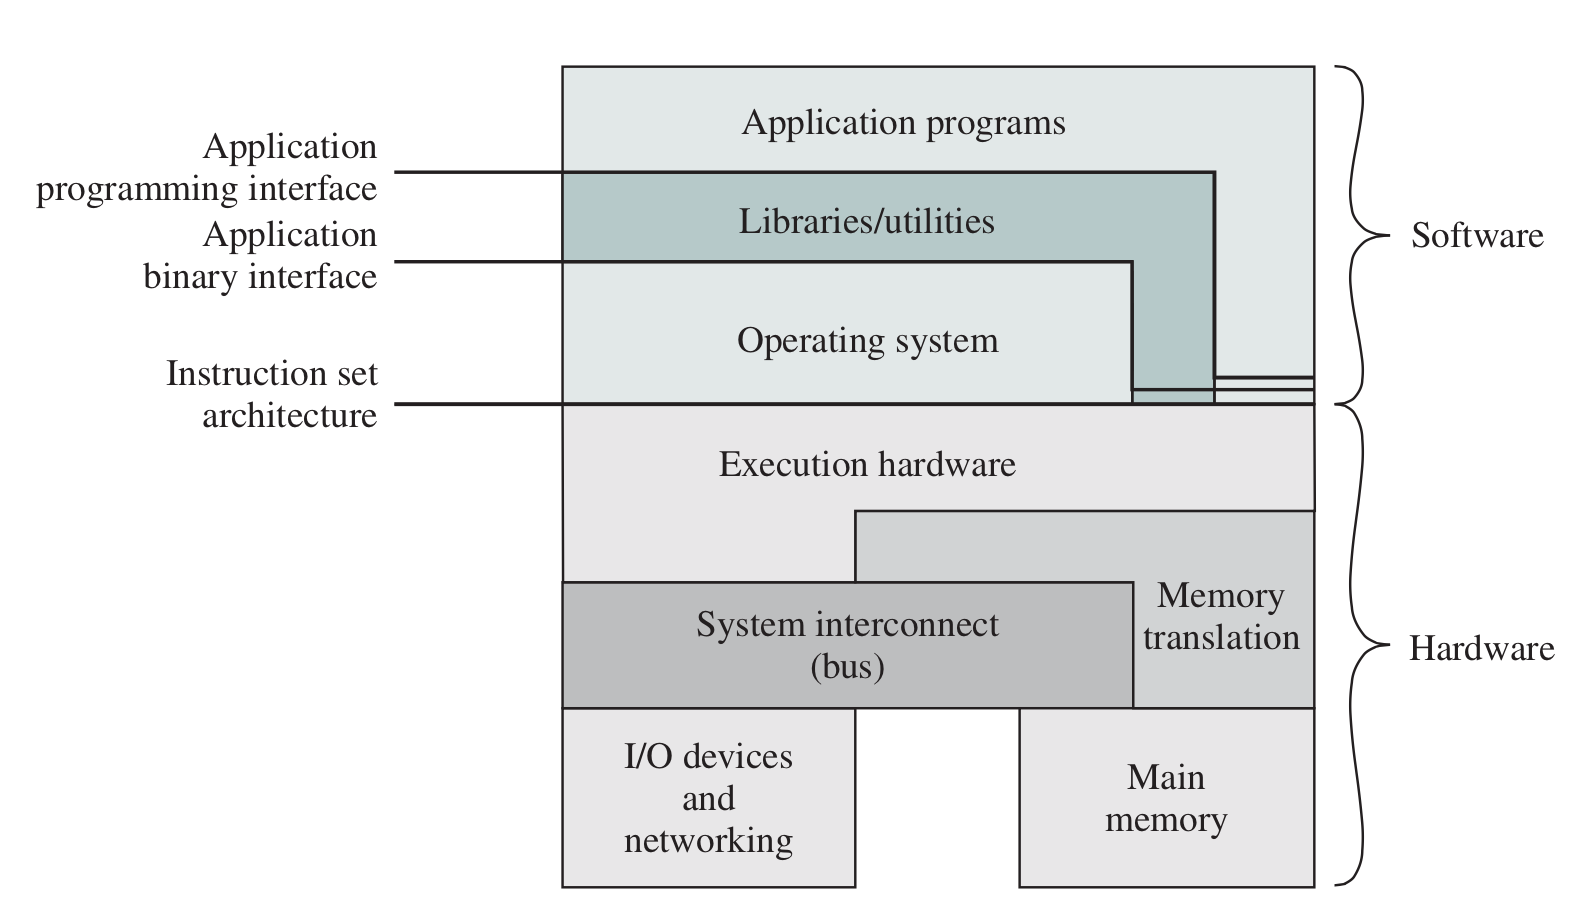
\includegraphics[width=0.73\textwidth]{images/os-sw-hw.png}\\
Structural diagram of a modern computer~\cite{osi}.
\end{center}

An operating system (often abbreviated OS) is a piece of software that sits between the hardware of a computer and the applications (programs) that run on that computer. The OS does many different things and often has many (occasionally-conflicting) goals. It is responsible for seeing to it that other programs can operate efficiently, providing an environment for other programs, and collecting and reporting data about what is and has been happening. It also needs to enforce policies that are defined by system administrators.

An operating system is also responsible for resource allocation. In the real world, the resources we have to work with, such as CPU time or memory space, are limited. The OS decides how to allocate these resources, keeps track of who currently owns what, and, in the event of conflicting requests, determines who gets the resource.

The OS usually enables useful programs like Photoshop or Microsoft Word to run. Any computer has various pieces of hardware, such as the CPU, memory, input/output devices (such as monitors, keyboards, modems). The OS is responsible for abstracting away the details of this, so that the authors of programs do not have to worry about the specifics of the hardware. Imagine how painful it would be to write even a simple program, like the Hello World example, if we had to write our program differently for every combination of hardware.

In most cases there will be multiple programs running on the computer. This implies the sharing of various resources. When this is the case, there is the potential for conflicts to arise. An operating system creates and enforces rules to make sure all the programs get along and play fairly. Of course, not all interaction between programs is competitive; sometimes they want to co-operate, and the OS helps them do that, too.

Another goal may be to use the computer hardware efficiently. This is not usually an issue with personal laptops, but imagine a supercomputer. A supercomputer used to do extremely complex computations is expensive to build and maintain. Any moment when the supercomputer is not doing useful work is a costly waste, so an operating system for such a computer would try to maximize CPU usage. There is, after all, only so much CPU time in supercomputers and there are many programs eager to run (weather simulations, particle physics simulations...).

Operating systems tend to be large and do a lot of things. We expect now that an OS comes with a web browser, an e-mail client, some method for editing text, et cetera. These things, while important and useful, are not what we are going to focus on. The part of the operating system that we will study is what we call the \textit{Kernel} - it is the ``core''; the portion of the OS that is always present in main memory and the central part that makes it all work.

Operating systems will evolve over time. There will be new hardware released, new types of hardware, new services added, and bug fixes. Evolution is constrained by a need to maintain compatibility for programs. If the user upgrades his or her desktop OS and a program breaks, even if it's the program author's fault, the user blames the OS vendor. If you look at Microsoft Windows, you can see their strict devotion to not breaking binary compatibility (at least, as much as they reasonably can). Linus Torvalds, yes, the person Linux is named after, gets unreasonably angry with people if they submit a kernel change that might break user-space programs. 

How obsessive are OS designers? Consider this example, admittedly from more than 25 years ago, about Windows 95 (yes, as in 1995)... from~\cite{joelce}:

\begin{quote}
Windows 95? No problem. Nice new 32 bit API, but it still ran old 16 bit software perfectly. Microsoft obsessed about this, spending a big chunk of change testing every old program they could find with Windows 95. Jon Ross, who wrote the original version of SimCity for Windows 3.x, told me that he accidentally left a bug in SimCity where he read memory that he had just freed. Yep. It worked fine on Windows 3.x, because the memory never went anywhere. Here's the amazing part: On beta versions of Windows 95, SimCity wasn't working in testing. Microsoft tracked down the bug and added specific code to Windows 95 that looks for SimCity. If it finds SimCity running, it runs the memory allocator in a special mode that doesn't free memory right away. That's the kind of obsession with backward compatibility that made people willing to upgrade to Windows 95.
\end{quote}

As we proceed we will focus on UNIX-like systems with some mention of Microsoft Windows where appropriate. This is for practical reasons: there is only so much time and UNIX-like systems represent a very large percentage of the operating systems out there including Linux, macOS/Mac OS X, Android, and more.

\section*{Time, What is Time?}
And then there's the real-time part of the puzzle. What makes a system real-time versus non-real-time? What it comes down to is whether or not wall-clock deadlines actually matter. Real life is full of systems, many of them embedded systems, that operate on the basis of meaningful deadlines. Some common examples of real-time systems include aviation, anti-lock braking systems, industrial machinery, video conferencing, and satellite launches.

When we talk about real-time systems, they deal with ``tasks'', which really are just things that need doing. Tasks are subdivided into the \textit{hard real-time} and \textit{soft real-time} categories. If a task is hard real-time, then a late answer is useless. If we're trying to launch a satellite into orbit, if the we don't have the calculation of when to fire the thrusters aren't ready in time, the calculation is not useful and would need to be repeated. If a task is soft real-time, then a late answer is of diminished quality but could still potentially be used: if decoding a frame of video takes longer than expected, the video quality (and viewing experience) is worse, but it's not totally ruined.

There will be much more about real-time systems later on. In most topics, we'll first talk about operating systems in general, and then we'll build on that to see what new complexity or differences the new constraint of real-time adds. 

\section*{Security Now}
When I taught a previous operating systems course, ECE 254, after the introduction, we spent some time talking about the history of operating systems and how we got to the modern generations of them. While some understanding of the history of a thing might be helpful in explaining some design decisions, the discussion was too vague and high-level to be useful. Nice trivia, maybe. So instead we are going to talk about security (but mostly, actually, protection).

In a lot of textbooks, security and protection are left to the end. This strikes me as being a problem: security is something you want to bake into your design and something you want to have in your mind constantly. It doesn't work to try to bolt it on afterwards. As we go through the topics of the course, we aren't going to stop at every opportunity to consider the security implications or risks of each implementation or decision... but it would still be a good idea to think about security in each situation.

An operating system is designed to support multiple users concurrently, each of whom are likely running multiple programs concurrently too. There are also the operating system's processes itself, which are not really under the user's control either. Even if you are the only user on your system, the operating system will enforce certain rules so that malicious programs (or malicious websites) can't steal your personal data or sabotage the system. 

Real-time operating systems are less likely than others to support the idea of multiple users concurrently; industrial machinery to assemble a tank doesn't really have user accounts and configuration the way that a server running Ubuntu might. Still, even that kind of system can have multiple processes concurrently -- user processes or OS processes -- so what we are discussing here is still relevant. 

Typically, OS designers create some policies and also policy tools. Some policies are just a part of the operating system and cannot be changed -- e.g., a file must have the ``execute'' permission to run. Others are configurable by system administrators -- e.g., may non-administrator users install new programs on the system? Security policies do have some tradeoff with usability, in that it can be frustrating for users who are denied some operation and must instead ask administrators to do it for them. But you also can't be too lax about this, because you most certainly do NOT want to find your company's name on TV having to report a data breach in which user personal data was stolen.

OS designers must see to it that the security policies (whether configured or not) are enforced consistently. This helps to ensure that sensitive data is protected, not corrupted, and only accessed by those who should have access. Operating systems that do not provide proper protection and security will inevitably be exploited by malicious users and it will cease to be used. 

Whatever the specifics about policies, there are three desirable properties that go by the acronym ``CIA'' -- Confidentiality, Integrity, Availability. Confidentiality is that information should only be access by those who are authorized to see it. Integrity is that information should be consistent and correct. Availability is that information or services should be available when they are needed.

\paragraph{Protection vs. Security} It's important to draw a quick distinction between \textit{protection} and \textit{security} as in~\cite{osc}. Protection is about ``internal threats'' -- things like making sure that user \texttt{morgan} cannot access the private files of user \texttt{taylor}. Security is more about ``external threats`` -- things like making sure that evil hackers don't gain access to the system. Maybe we take those in order.

\subsection*{Protection}
Truthfully, most of our discussion in this course will be about protection -- how does the design of the operating system ensure that the rules are followed. Following the rules is important to actually have a functioning system. Without it, anarchy results. As much as we'd all like to live in a world where everyone is nice and nobody does anything wrong, but, uh, have you seen the news? But even if you did have a system where all the legitimate users lacked malicious intent, it would be possible for someone to disrupt the experience of others by accident. That sometimes happens on the ECE-operated servers, where someone unintentionally writes a program that exhausts shared memory or gets in an infinite loop and uses excessive CPU time.

What are the goals, then, of protection? Ultimately, it's about enforcing the policies about responsible resource usage~\cite{osc}. What is responsible and reasonable for a given system may be different when compared to a different system. Some servers are dedicated to running exactly one service and there's nothing wrong with letting that service take all available CPU time, memory, disk space... Other servers, like the ECE Ubuntu systems, are meant to be shared amongst hundreds and hundreds of students, any of whom could be working on different courses at any time... so resources there need to be shared. 

An obvious case of access control that's important to consider is permissions on files. There are many files in a shared system, but not all of them are yours. Some of them belong to you, yes, and some belong to other users, and yet others belong to the operating system itself. You wouldn't want to do your assignment on a shared server that had no enforcement of ownership: it would be all too easy for someone to copy your code... or delete it to sabotage you. 

Another example: the operating system also enforces logical walls between different processes. As we go through the course we'll see a few different cases. For one, the memory of a given program is not accessible with other programs.

These rules take some effort to enforce: requests and actions have to be checked, by the operating system (of course), to make sure that they are valid, where valid means in compliance with the rules.

With that said, there are exceptions. You can make a file ``public'' so that you would intentionally allow others to access it. You can also ask your program to used shared memory such that another program can share the same section (and we'll talk about that). Also, system administrators can generally override policies and do things that normal users can't... including reading other people's files. You can see why we need a lot of trust in administrators.

The usual protection rules that we see above -- limiting access to data based on rules -- are the most common ones, but they aren't the only ones. We could have rules that terminate processes if they use too much CPU time or memory, but those are fairly rare in the real world. While there are probably no good reasons for users to read one another's data, there are frequently good reasons for using a lot of resources. 

Let's imagine for a minute that I want to edit a lecture video. It makes sense, then, that editing the video uses a very large amount of memory as I'm putting together all the different pieces of content. When I'm done editing and I want to render the video (create the final video output), that's a CPU-intensive task and it may max out all the CPUs for quite a while. That's a perfectly legitimate use of the system -- I'm not doing anything malicious and it's for a valid work-related purpose. But it would maybe set off alarms if we just considered the memory and/or CPU usage in isolation.

That does mean that people can exploit the lack of strictness and make excessive use of system resources. When we talk about scheduling algorithms, we'll see how a real system will do its best to make sure that even if a user is requesting excessive CPU time, that it won't impact others excessively. If that's not enough, there's always the option to escalate to system administrators who can do something about it.

So this brief introduction should hopefully make clear the importance of protection when we consider how file systems, shared memory, and others work to prevent internal problems... so let's also consider external factors.

\subsection*{Security}
Although we won't talk about security in as much detail as protection, I want to at least go over a few different ways in which attackers could try to exploit the system. We need this in mind when understanding the design of an operating system because the presence of these threats will cause us to change how we design systems. Just think about how different air travel would be if there were actually no need for security. 

Some attacks worth considering below~\cite{osc}:
\begin{itemize}
	\item \textbf{Breach of Confidentiality.} This is when some external actor gains access to information they should not be able to have, such as users' personal details (name, address, etc) or private information (health records, financial records). Getting this data is pretty lucrative for attackers, because it can be used for the attacker's financial gain. It's also terrible for the company, because a leak of private information makes regulatory authorities very mad.
	
	\item \textbf{Breach of Integrity.} This is when an attacker is able to corrupt or otherwise alter data that they should not have access to. This can be totally destructive -- erase all users from the database -- or more subtle, where the attacker increases the payroll pay going to a certain account. 
	
	\item \textbf{Theft of Service.} This is what happens when an attacker is able to make use of some resources that they should not be able to. This might be getting some paid software-as-a-service without paying, or using the company servers to mine cryptocurrency, for example.
	
	\item \textbf{Breach of Availability and Denial of Service.} This is what happens when an attacker is able to prevent a service from working as intended. This might be by trying to overwhelm a service with too many requests, or it could be deliberately crashing a server that is vulnerable in some way. 
	
\end{itemize}

These categories are not exhaustive, but give an idea of the kind of bad behaviour that we should be worried about. If we want to have a secure system, good design of the operating system is necessary but not sufficient. If a house has locks but the owners don't use them, the locks are not very effective. Configuration and policies are important too. But there's also the human factor.

Most likely the weakest link in any system is the human! A perfectly secure system technically can easily be defeated by \textit{phishing}, an attacker tricking a legitimate user into handing over their credentials or doing something they should otherwise not be doing (``yes, I'll tell you the payroll information...''). That sort of thing is harder to design to solve, but should not be overlooked either.

The categories discussed above are just types of problem that attackers can cause. Some of them used examples where I gave a specific type of attack, but here's a few ideas, not exhaustive (obviously) that come to mind:

\begin{itemize}
	\item \textbf{Excessive Requests} -- overload the system with demands, whether for CPU, memory, responses, etc.
	\item \textbf{Malformed Requests} -- send intentionally malformed requests that can cause the system to behave in an unexpected way, crash, or return information it should not be sending.
	\item \textbf{Back Door} -- sneaking some code into a program that allows (normally unauthorized) access to a system
	\item \textbf{Intercepting Messages} -- observing the communication between systems and intercepting messages to change them or gain information. This is also called a Man-in-the-Middle Attack.
	\item \textbf{Trojan Horse} -- tricking someone into installing something that contains a hidden payload that can do one of the things above...
\end{itemize}

Security is, and always has been, a sort of arms race. When an exploit or other vulnerability is discovered, operating system developers need to find a way to guard against it and implement a patch for it (and roll it out). Sometimes the security problem is just the result of a bug, in which case patching it just ensures the system has its intended behaviour. If it's a design problem, then changing the design might actually be painful because it will cause existing software to break. It gets worse, I suppose, because if a bug has been around for long enough, programs may actually rely on the behaviour of that bug. So patching it breaks them too!

Now we have a dilemma! What do we do? Break existing software in the name of security or preserve the user-land programs' behaviour at the cost of security? There are no one-size-fits all answers to this question. That would be too easy.

This is not a course in security, so we can't spend too much time talking about it and will cut it off here, even if it can be fascinating. The goal is that we should just be thinking about security (and protection) when considering a design decision. And that consideration should take place early on in the process and not be simply an afterthought!

\bibliographystyle{alphaurl}
\bibliography{350}


\end{document}